\documentclass[Charts101.tex]{subfiles}
\begin{document}
\begin{frame}
\frametitle{U-Charts}	
\large
\begin{itemize}
\item In statistical quality control, the c-chart is a type of control chart used to monitor "count"-type data, typically total number of nonconformities per unit.[1] 
\item It is also occasionally used to monitor the total number of events occurring in a given unit of time.
\end{itemize}

\end{frame}
%==================================================================== %
\begin{frame}
	\frametitle{C-Charts}
	\Large
	
	\begin{figure}
\centering
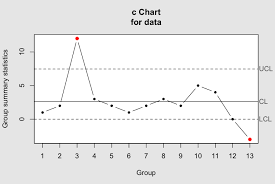
\includegraphics[width=1.0\linewidth]{C-chart}

\end{figure}

\end{frame}
%==================================================================== %
\begin{frame}
\frametitle{C-Charts}
\Large
\begin{itemize}
\item The c-chart differs from the p-chart in that it accounts for the possibility of more than one nonconformity per inspection unit, and that (unlike the p-chart and u-chart) it requires a fixed sample size. 
\item The p-chart models "pass"/"fail"-type inspection only, while the c-chart (and u-chart) give the ability to distinguish between (for example) 2 items which fail inspection because of one fault each and the same two items failing inspection with 5 faults each; in the former case, the p-chart will show two non-conformant items, while the c-chart will show 10 faults.
\end{itemize}


\end{frame}
%==================================================================== %
\begin{frame}
\frametitle{C-Charts}
\Large
Nonconformities may also be tracked by type or location which can prove helpful in tracking down assignable causes.

Examples of processes suitable for monitoring with a c-chart include:
\begin{itemize}
\item[$\ast$] Monitoring the number of voids per inspection unit in injection molding or casting processes
\item[$\ast$] Monitoring the number of discrete components that must be re-soldered per printed circuit board
\item[$\ast$] Monitoring the number of product returns per day
\end{itemize}

\end{frame}
%==================================================================== %
\begin{frame}
\frametitle{C-Charts}
\Large
The Poisson distribution is the basis for the chart and requires the following assumptions:
\begin{itemize}
\item 
The number of opportunities or potential locations for nonconformities is very large
\item The probability of nonconformity at any location is small and constant
\item The inspection procedure is same for each sample and is carried out consistently from sample to sample
\end{itemize}

\end{frame}
%==================================================================== %
\begin{frame}
\frametitle{C-Charts}
\Large

The control limits for this chart type are \[ \bar{c} \pm 3\sqrt{\bar{c}}\] where $\bar{c}$ is the estimate of the long-term process mean established during control-chart setup.


\end{frame}
%==================================================================== %
\end{document}